\documentclass[tikz,border=2pt]{standalone}
\usepackage{xcolor}
\begin{document}
% III_0D
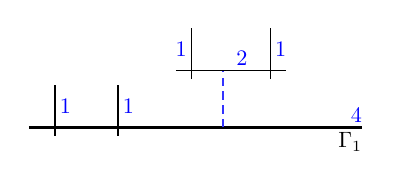
\begin{tikzpicture}[xscale=1,yscale=0.9]
\draw[thick,shorten >=2] (-1/3,0)--(119/30,0) node[inner sep=2pt,blue,above left,scale=0.8] {4} node[inner sep=2pt,below left,scale=0.8] {$\Gamma_1$};
\draw[shorten <=-3pt] (0,0)--node[inner sep=2pt,scale=0.8,blue,right] {1} (0,3/5);
\draw[shorten <=-3pt] (4/5,0)--node[inner sep=2pt,scale=0.8,blue,right] {1} (4/5,3/5);
\draw[blue!80!white,densely dashed] (32/15,0)--(32/15,4/5);
\draw (23/15,4/5)--node[inner sep=2pt,scale=0.8,blue,above,pos=0.6] {2} (44/15,4/5);
\draw[shorten <=-3pt] (26/15,4/5)--node[inner sep=2pt,scale=0.8,blue,left] {1} (26/15,7/5);
\draw[shorten <=-3pt] (41/15,4/5)--node[inner sep=2pt,scale=0.8,blue,right] {1} (41/15,7/5);
\end{tikzpicture}
\end{document}
